\cleardoublepage
\chapter{Theoretical background\label{ch:theoretical-background}}

In this chapter, we give an overview of the main methods -- and the theory behind -- used nowadays in computational physics to evaluate the electronic structure of materials. In particular, the focus will be on spectral properties, and on the possibilities and limitations that the discussed approaches have both at an exact level and in practical applications. The \emph{leitmotiv} of this chapter is the nature of the effective interaction felt by an electron, as a consequence of the interplay with the rest of the system. Starting from standard density-functional theory, Sec.~\ref{sec:dft}, we discuss the physical meaning of the Kohn-Sham auxiliary system characterized by a static and local potential; we also go through some fundamental properties of the exact energy functional and their validity within the context of current (local and semi-local) approximations. In Sec.~\ref{sec:non-local}, we consider non-local hybrid functionals which embody part of the Fock exchange in the effective potential. Finally, in Sec.~\ref{sec:green-function-methods}, we point out the main features of Green's function-based methods bringing about the concept of self-energy, a non-local and dynamical potential that, ultimately, accounts for all the electronic correlations via a single-particle picture. In Sec.~\ref{sec:ch2-summary}, we summarize the key messages of the chapter.

\clearpage
\section{Density-functional theory\label{sec:dft}}
Density-functional theory (DFT) is the most popular and widely used method for electronic structure calculations \cite{van_noorden_top_2014}. The secret behind the success of this theory lies in the dramatically reduced computational complexity of the many-electron problem: rather than describing the electrons in terms of the wave function $\Psi$ (see Eq.~\eqref{eq:many-electron-problem}) -- characterized, for a $N$-electron system, by $3N$ degrees of freedom -- all the many-electron quantities are expressed as functionals of the total electronic density $\rho(\br)$. As a consequence, regardless the number of electrons in the system, the number of degrees of freedom reduces to three. On the other hand, we lose track of the individual electronic coordinates and we embrace a description where the electrons are considered as a whole, which sometimes makes more difficult to understand the nature of the interaction -- as well as the possible errors (e.g. the self-interaction error discussed in Sec.~\ref{sec:errors-dft}) -- embodied by actual functionals.

While the founding pillars of DFT are the two Hohenberg-Kohn theorems, it is thanks to the Kohn-Sham auxiliary system that we an effective way to tackle the problem; this is discussed in Sec.~\ref{sec:hk-ks-theorems}. In Sec.~\ref{sec:dft-approx}, we introduce local and semi-local approximations to the unknown exchange-correlation energy functional, which paved the way to electronic structure calculations. The piecewise-linearity of the ground-state energy, the derivative discontinuity and the band gap problem in DFT are discussed in Secs.~\ref{sec:pwl-energy} and \ref{sec:deriv-dis}. Finally, in Sec.~\ref{sec:errors-dft}, we analyze the main errors of density-functional approximations and how to some possible ways to overcome them.

\subsection{HK theorem and the KS mapping\label{sec:hk-ks-theorems}}
The work from Hohenberg and Kohn (HK), published in 1964 \cite{hohenberg_inhomogeneous_1964}, shows that the electronic energy is a unique functional of the total density and has the property of being variational. By referring to Eq.~\eqref{eq:many-electron-problem}, we define $\{ \hat{V} \}$ as the set of all the possible local one-particle potentials (considered non-equivalent only if they differ by more than a constant), and $\{ \Psi \}$ and $\{ \rho \}$ as the set of all the ground-state ($N$-body) wave functions and densities, respectively. In the first part of their theorem, HK show that there exists an invertible map connecting the elements of $\{ \hat{V} \}$ to the elements of $\{ \Psi \}$ and, even more importantly, to those of $\{ \rho \}$:
%
\begin{equation}
    \{ \hat{V} \} \curvedrightleft \{ \Psi \} \curvedrightleft \{ \rho \} .
    \label{eq:hk-theorem}
\end{equation}
%
While the original proof of the theorem was restricted to non-degenerate ground states, the generalization to degenerate states can be found in Ref. \cite{dreizler_density_1990}. Making use of the result above, in the second part of the theorem, HK define for a fixed potential $\hat{V} \in \{ \hat{V} \}$ the following functional:
%
\begin{equation}
\begin{split}
    E[\rho] &= \braket{\Psi[\rho]|\hat{T} + \hat{V}_{\rm ee} + \hat{V}|\Psi[\rho]} \\
    &= F^{\rm HK}[\rho] + \int d\br v(\br) \rho(\br) ,
\end{split}
\label{eq:hk-functional}
\end{equation}
%
where $F^{\rm HK}[\rho]$ is a universal functional of the density, in the sense that it does not depend on the external potential $\hat{V}$, and is unambiguously defined only by the number of electrons in the system. Thanks to the Rayleigh-Ritz principle, the energy correspondent to the density $\rho$, connected to $\hat{V}$ via the map \eqref{eq:hk-theorem}, is a lower bound for the functional $E[\rho]$. The ground state energy of an electronic system can then be found by searching, over all the possible $v$-representable\footnote{These are all the densities that correspond to some element of $\{ \hat{V} \}$; an extension of the theorem to densities that are not $v$-representable, but simply $N$-representable, which means that they correspond to some $N$-particle antisymmetric wave function, has been showed later by Levy \cite{levy_electron_1982} and Lieb \cite{shimony_physics_1982}.} densities, the one that minimizes the functional of Eq.~\eqref{eq:hk-functional}.

HK theorem provides a framework for the search of the ground state of many-electron systems, but it does not show how to build the map \eqref{eq:hk-theorem} or give an explicit definition of the functional $F^{\rm HK}[\rho]$. In 1965, Kohn and Sham (KS) assumed the existence of a single-particle, local, mean-field approach sharing the same ground-state density of the real system \cite{kohn_self-consistent_1965}. They started defining the density from a set of one-particle orthonormal orbitals $\phi_i(\br)$ as
%
\begin{equation}
    \rho(\br) = \sum_i^{\rm occ} \phi^*_i(\br) \phi_i(\br) ,
    \label{eq:density}
\end{equation}
%
and introduced a new quantity called exchange-correlation (xc) energy, $E_{\rm xc}$, embodying all the ``non-explicit'' part of the electronic interactions:
%
\begin{equation}
    E[\rho] = T_0[\rho] + E_{\rm H}[\rho] + E_{\rm xc}[\rho] + V[\rho] ;
    \label{eq:energy-functional}
\end{equation}
%
by comparison with Eq.~\eqref{eq:hk-functional}, we see that
%
\begin{equation}
    E_{\rm xc}[\rho] = T[\rho] - T_0[\rho] + V_{\rm ee}[\rho] - E_{\rm H}[\rho] ,
    \label{eq:xc-energy}
\end{equation}
%
where $T_0$ is the non-interacting kinetic energy
%
\begin{equation}
    T_0[\rho] = \sum_i \braket{\phi_i | -\nabla^2/2 | \phi_i} ,
    \label{eq:non-int-kinetic}
\end{equation}
%
and $E_{\rm H}$ is the Hartree energy
\begin{equation}
    E_{\rm H}[\rho] = \frac{1}{2} \int d\br d\br' \frac{\rho(\br)\rho(\br')}{|\br-\br'|} .
    \label{eq:hartree-energy}
\end{equation}
%
By means of the HK variational principle, one can find the stationary points of the energy functional upon variation with respect to the one-particle orbitals $\phi_i$ (while enforcing the orthonormality constraint on the orbitals). As a result, we find the following set of equations that, together with Eq.~\eqref{eq:density}, take the name of \emph{KS equations}:
%
\begin{equation}
    \left[ - \frac{\nabla^2}{2} + v_{\rm H}([\rho],\br) + v_{\rm xc}([\rho],\br) + v(\br) \right] \phi_i(\br) = \varepsilon_i \phi_i(\br) .
    \label{eq:ks-equations}
\end{equation}
%
The sum of the three potentials $v_{\rm H}([\rho],\br) + v_{\rm xc}([\rho],\br) + v(\br)$ yields the effective potential $v_{\rm eff}(\br)$, where $v_{\rm H}$ is the functional derivative of the Hartree energy, also known as Hartree potential,
%
\begin{equation}
    v_{\rm H}([\rho],\br) = \frac{\delta E_{\rm H}[\rho]}{\delta \rho(\br)} = \int d\br' \frac{\rho(\br')}{|\br - \br'|} ,
    \label{eq:hartree-potential}
\end{equation}
%
and $v_{\rm xc}$ is the functional derivative of the exchange-correlation energy, also know as xc potential,
%
\begin{equation}
    v_{\rm xc}([\rho],\br) = \frac{\delta E_{\rm xc}[\rho]}{\delta \rho(\br)} .
    \label{eq:xc-potential}
\end{equation}
%
An important feature of Eq.~\eqref{eq:ks-equations} is the dependency of the Hamiltonian -- through the density $\rho$ -- on its own eigenvectors, which makes the KS equations \emph{almost} an eigenvalue problem. The stationary points of the energy functional, i.e. the ground state of the system, can be found via a self-consistent field solution of the KS equations, and it is only at self-consistency that: (i) the dependency of the Hamiltonian on the density $\rho$ disappears, (ii) the effective potential $v_{\rm eff}(\br)$ becomes the KS potential $v_{\rm KS}(\br)$, and (iii) the KS equations become an eigenvalue problem.

Here we point out that, as a consequence of HK theorem, the electronic ground-state density determines univocally also the many-body Hamiltonian of the system. The sets of eigenvalues and eigenvectors are also in a one-to-one correspondence with the density, and thus are all the properties that can be derived from them (including excited-state properties). The main issue then, is to find a way to calculate those quantities once the density is known, which means to determine the explicit expression for the map connecting the properties of the system to its ground-state density. The KS mapping provides a way to obtain the real ground-state density only, by looking at an auxiliary system of non-interacting electrons. Other than the electronic density, there is no theorem that proves that the properties of the KS system (orbital energies, wave functions, total energies, \dots) have any actual physical meaning \cite{martin_interacting_2016}. The only other exception is represented by the highest-occupied (HO) energy level, $\varepsilon_{\rm HO}$, which corresponds to the opposite of the ionization potential (IP), $E(N-1) - E(N)$, of the real system. This has been shown by Perdew \emph{et al.} \cite{perdew_density-functional_1982} to be a consequence of the property of the ground-state energy of being a piecewise-linear function of the number of electrons (see discussion in Sec.~\ref{sec:pwl-energy}). But, in a more straightforward way, can also be proven by looking at the behavior of the density far from the system: as shown by Almbladh and von Barth \cite{almbladh_exact_1985}, as $|\br| \longrightarrow \infty$, the ground-state density decays asymptotically as
%
\begin{equation}
    \rho(\br) \sim e^{-2\sqrt{-2\mu}|\br|} ,
    \label{eq:exp-decay-density}
\end{equation}
%
where $\mu$ represents the chemical potential which corresponds to the opposite of the ionization potential. Since the density of the KS system matches that of the real system, also the asymptotic behavior must be identical. One concludes that the IPs of the KS and of the real system are the same, and given that the IP of the KS system is equal to $-\varepsilon_{\rm HO}$, we finally obtain
%
\begin{equation}
    \varepsilon_{\rm HO} = E(N) - E(N-1) .
    \label{eq:ip-theorem}
\end{equation}
%
Eq.~\eqref{eq:ip-theorem} is known as \emph{IP-theorem}, or \emph{DFT Koopmans' theorem}, to not be confused with the original Koopmans' theorem \cite{koopmans_uber_1934}, formulated within the framework of Hartree-Fock theory (see Sec.~\ref{sec:hartree-fock}). With respect to Hartree-Fock, where the connection between eigenvalues and photoemission energies applies to the whole spectrum, in DFT this result regards only the HO state; on the other hand, the silver lining is that Eq.~\eqref{eq:ip-theorem} is approximation-free and it is valid in the framework of exact DFT, while the original Koopmans' theorem works only for the Hartree-Fock system -- where electronic correlation is totally absent -- and the orbitals relaxation, upon addition of holes or electrons, is neglected.

Some efforts have been done in order to give a rigorous justification for the interpretation of the KS states as quasiparticles of the real system. It has been argued that the KS eigenvalues might represent a first-order approximation to the vertical excitation energies \cite{chong_interpretation_2002} and, indeed, it seems that close to the Fermi level the differences between the many-body self-energy and the xc potential tend to be small (at least for the homogeneous electron gas) \cite{jones_density_1989}. Similar arguments could be used for KS and Dyson orbitals. Yet, no formal connection has been found for the moment \cite{di_valentin_gas-phase_2014}, and the only situation where the KS states provide vertical excitation energies and Dyson orbitals is for non-interacting systems.

\subsubsection*{Janak's theorem}
An important result regarding the orbital energies has been proposed by Janak in 1978 \cite{janak_proof_1978_corrected}, and it is going to be used often throughout this work. In his paper, Janak showed that the eigenvalues $\varepsilon_i$ satisfy the following property:
%
\begin{equation}
    \frac{dE}{df_i} = \varepsilon_i ,
    \label{eq:janak-th}
\end{equation}
%
where $f_i$ is the occupation number of the $i$-th orbital. While this is certainly valid for the HO state (see also Sec.~\ref{sec:pwl-energy}), for the other orbitals it passes through the definition of an energy functional which is not strictly equal to the HK one. In this generalized framework, the kinetic energy functional differs from its original definition,
%
\begin{equation}
    \Tilde{T} = \sum_i f_i \braket{\phi_i| -\nabla^2/2 |\phi_i} ,
    \label{eq:janak-kinetic}
\end{equation}
%
and also the electronic density is redefined in order to include the occupation numbers,
%
\begin{equation}
    \rho(\br) = \sum_i f_i |\phi_i(\br)|^2 .
    \label{eq:janak-density}
\end{equation}
%
The $f_i$ are treated as parameters taking any values between 0 and 1, and it is only in the special case where they follow the Fermi-Dirac distribution, that the density and the kinetic energy recover the expressions of Eqs.~\eqref{eq:density} and \eqref{eq:non-int-kinetic}, respectively, and we find again the HK energy. Therefore, with the exception of the HO orbital, Eq.~\eqref{eq:janak-th} cannot be strictly considered a result within the domain of DFT, yet it is useful when considering beyond-DFT approaches that want to treat the electronic occupations as parameters.

\subsection{Local and semi-local approximations\label{sec:dft-approx}}
The KS mapping defines a way to tackle the variational problem defined by HK, however, in order to solve the KS equations, one needs to know the functional dependency of the xc energy on the density. The exact expression is generally not known, thus approximations are needed. The oldest approximation for the xc energy, already proposed by Kohn and Sham in 1965 \cite{kohn_self-consistent_1965}, is the local-density approximation (LDA), which takes the expression for the xc energy of the homogeneous electron gas (HEG) at any value of the density $\rho(\br)$:
%
\begin{equation}
    E_{\rm xc}[\rho] = \int d\br \rho(\br) \varepsilon^{\rm HEG}_{\rm xc}(\rho(\br)) .
    \label{eq:lda-xc}
\end{equation}
%
The xc energy density can be decomposed in its exchange and correlation parts, $\varepsilon^{\rm HEG}_{\rm xc} = \varepsilon^{\rm HEG}_{\rm x} + \varepsilon^{\rm HEG}_{\rm c}$, where the exchange term has the following analytical expression
%
\begin{equation}
    \varepsilon^{\rm HEG}_{\rm x}(\rho) = - \frac{3}{4} \left( \frac{3\rho}{\pi} \right)^{\frac{1}{3}} ,
    \label{eq:lda-ex}
\end{equation}
%
while the correlation term has been numerically computed by Ceperley and Alder \cite{ceperley_ground_1980}, and later parameterized in terms of the Wigner-Seitz radius $r_{\rm s}$ by Perdew and Zunger \cite{perdew_self-interaction_1981}:
%
\begin{equation}
    \varepsilon^{\rm HEG}_{\rm c}(r_{\rm s}) =
    \begin{cases}
        -0.1423 / \left( 1 + 1.0529\sqrt{r_{\rm s}} + 0.3334 r_{\rm s} \right) & \text{for} \quad r_{\rm s} \geq 1 \\
        0.0311 \ln(r_{\rm s}) - 0.048 + 0.002 r_{\rm s} \ln(r_{\rm s}) - 0.0116 r_{\rm s} \qquad & \text{for} \quad r_{\rm s} < 1
    \end{cases} .
    \label{eq:lda-corr}
\end{equation}

The success of LDA, even for non-homogeneous systems, is probably due to the fact that some important exact constraints are satisfied like, e.g., the sum rule on the exchange-correlation hole. Still the totally local nature of the approximation, makes it neglect the effects of the spatial variations of the density around any point $\br$. Hence, the obvious next step to improve LDA is to account for the first-order spatial variations, i.e. the gradient, of the density. Generalized-gradient approximations (GGAs) are then given defined as
%
\begin{equation}
    E^{\rm GGA}_{\rm xc}[\rho] = \int d\br \varepsilon^{\rm GGA}_{\rm xc}(\rho(\br), \nabla\rho(\br)) .
    \label{eq:gga-xc}
\end{equation}
%
The most famous and used GGA functional is the Perdew-Burke-Ernzerhof (PBE) functional \cite{perdew_generalized_1996}, which is also the base functional used for all the calculations in this thesis. Following the same strategy, one could continue to add higher-order derivatives of the density; meta-GGA functionals include also second-order gradients, as well as other semi-local quantities such as the kinetic energy densities and thus sit on a higher rung in Jacob's ladder \cite{perdew_jacobs_2001}. Among all the different recipes, here we mention the Strongly-Constrained and Appropriately-Normed (SCAN) functional \cite{sun_accurate_2016}, that with its 17 exact constraints fulfilled is one of the most accurate semi-local approximations.

\subsection{Piecewise-linearity of the ground-state energy\label{sec:pwl-energy}}
In 1982, Perdew \emph{et al.} \cite{perdew_density-functional_1982} discovered a fundamental property of the exact ground-state energy of an electronic system, which represents one of the main concepts driving the formulation of Koopmans-compliant functionals. As a function of the number of electrons, the energy is piecewise-linear (see Fig.~\ref{fig:pwl}), which means that: (i) it is linear between integer points, and (ii) its first derivative has a discontinuity when passing through an integer number of electrons.

The first part of the proof involves a generalization of the energy functional to fractional particle numbers. Let us consider a density $\rho(\br)$ that integrates to $N=M+\delta$, where $M$ is an integer number and $\delta$ is a real number between 0 and 1. Such a density cannot correspond to a pure state, therefore one needs to resort to density matrices mixing integer-particle states:
%
\begin{equation}
    \hat{\rho} = \sum_i \alpha_i \ket{\Psi_i}\bra{\Psi_i} \qquad \qquad \text{with} \qquad
    \sum_i \alpha_i = 1 ,
    \label{eq:mixed-state}
\end{equation}
%
where, in this picture, $\Psi_i$ is a $i$-particle wave function and $\alpha_i$ are mixing parameters. In order to define the energy functional, one must search over all the density operators $\hat{\rho}$ giving the density $\rho(\br)$; the expectation value of the Hamiltonian, showed in Eq.~\eqref{eq:energy-functional}, becomes an ensemble average where the external potential reduces to the same expression given in Eq.~\eqref{eq:energy-functional}, while the universal functional is defined as
%
\begin{equation}
    F^{\rm HK}[\rho] = \min_{\hat{\rho} \longrightarrow \rho(\br)} {\rm tr} \left\{ \hat{\rho} \left( \hat{T} + \hat{V}_{\rm ee} \right) \right\} .
    \label{eq:energy-general-mixture}
\end{equation}
%
For simplicity, one normally considers a statistical mixture involving only the $M$- and the $(M+1)$-electron density operators and the energy minimization problem reduces to
%
\begin{equation}
    E_0 = \min_{\substack{\rho(\br) \\ \int d\br \rho(\br) = M+\delta}} \min_{\Psi_M, \Psi_{M+1}}
    \left[ (1-\delta) \braket{\Psi_M|\hat{H}|\Psi_M} + \delta \braket{\Psi_{M+1}|\hat{H}|\Psi_{M+1}} \right] ,
    \label{eq:pwl-energy-min}
\end{equation}
%
where $\alpha_{M} = 1 - \delta$ and $\alpha_{M+1} = \delta$, as a consequence of the normalization condition on the mixing parameters and of the normalization to $M+\delta$ of the density\footnote{Thanks to the convexity of the energy with respect to the mixing parameters, the same result is obtained when starting from the more general ensemble average given in Eq.~\eqref{eq:energy-general-mixture}.}. The minimum is trivially obtained for $\Psi_M$ and $\Psi_{M+1}$ being the ground states of the $M$- and $(M+1)$-electron systems. The solution of Eq.~\eqref{eq:pwl-energy-min} yields
%
\begin{equation}
    E_0 = (1 - \delta) E_M + \delta E_{M+1} ,
    \label{eq:pwl-energy}
\end{equation}
%
which shows that the ground-state energy is a linear function of $N$, for $M \leq N \leq M+1$.

The second part of the proof consists of proving that the derivative of $E(N)$, i.e. the chemical potential $\mu(N)$, has discontinuous jumps when passing through an integer $N$. The demonstration, by \emph{reductio ad absurdum}, comes once more from Ref.~\cite{perdew_density-functional_1982}. Let us consider two atoms from different chemical species, $X$ and $Y$, such that $\mu(Y)<\mu(X)$. When they are far apart, the two atoms do not interact and the total energy is simply given by the sum of the energies of $X$ and $Y$. If we now imagine a small fraction of an electron $\delta N$ moving from $X$ ($\delta N_X = - \delta N < 0$) to $Y$ ($\delta N_Y = \delta N > 0$), the net change of energy will be
%
\begin{equation}
    [\mu(Y) - \mu(X)] \delta N < 0 .
    \label{eq:proof-discontinuity-mu}
\end{equation}
%
Therefore, if $\mu(N)$ were a continuous function of $N$, for any pair of atoms a small fluctuation in the density would lead to more energetically favorable state where both the atoms are ionized. The discontinuity of the chemical potential, when passing through an integer $N$, solves this paradox; by using Eq.~\eqref{eq:pwl-energy}, we conclude that
%
\begin{equation}
    \mu(N) =
    \begin{cases}
        E(M) - E(M-1) \qquad \text{for} \quad M-1<N<M \\
        E(M+1) - E(M) \qquad \text{for} \quad M<N<M+1
    \end{cases}
    \label{eq:mu-ip-ea}
\end{equation}
%
where the first line gives the (opposite) ionization potential, $I(M)$, introduced earlier, and the quantity in the second line is the (opposite) electron affinity (EA), $A(M)$. Finally, we point out that among all the elements largest EA (chlorine) is 3.62 eV and it is still smaller than the lowest IP (caesium), 3.89 eV, which makes Eq.~\eqref{eq:proof-discontinuity-mu} never true for neutral atoms.
%
\begin{figure}
    \centering
    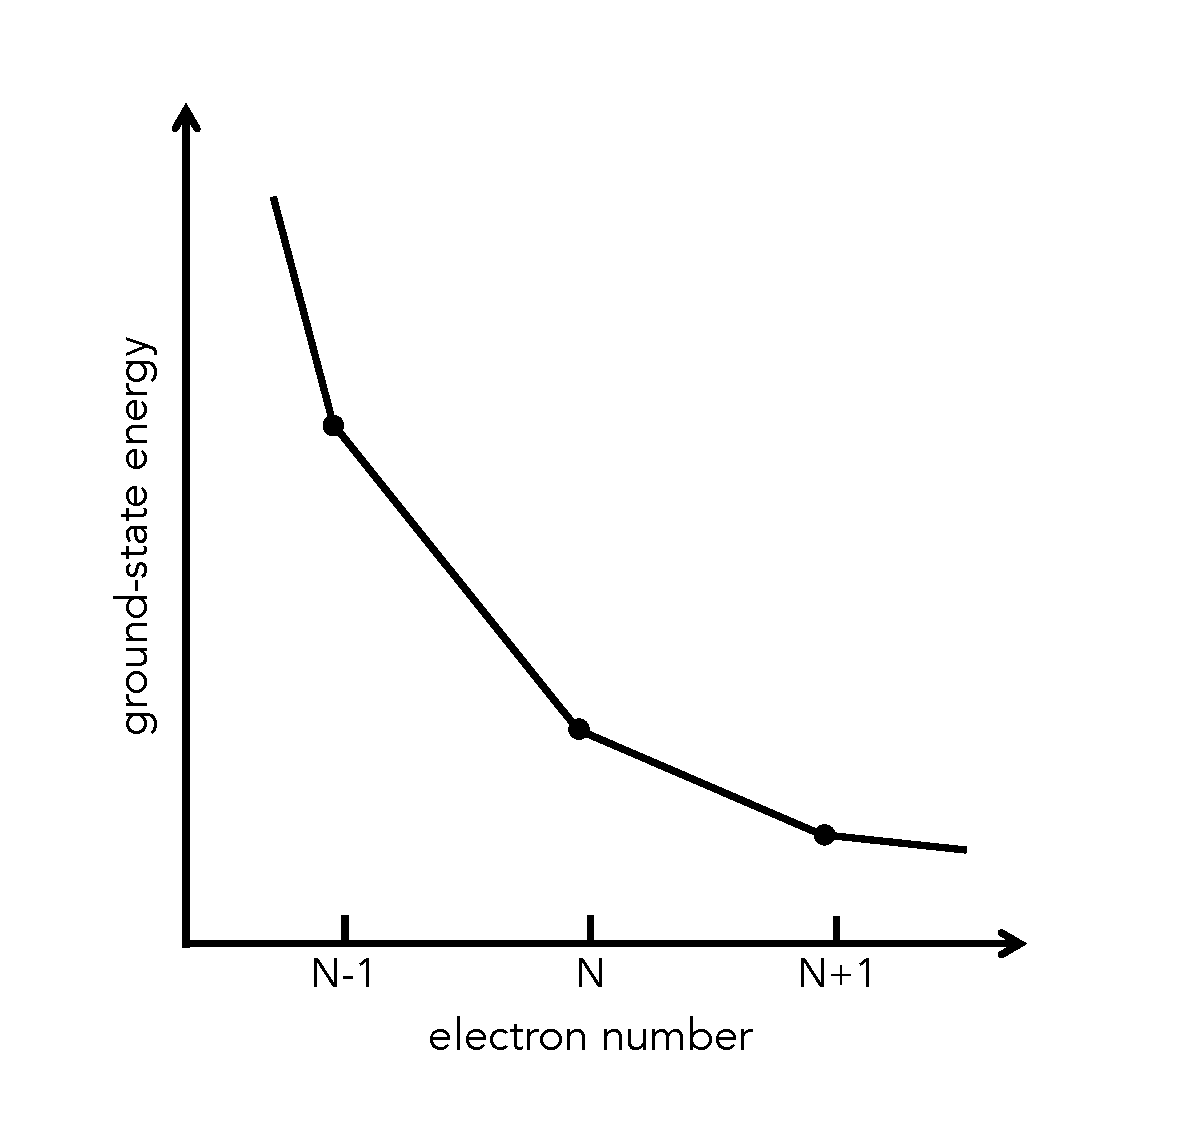
\includegraphics[width=0.5\textwidth]{pwl-exact.pdf}
    \caption{Ground-state energy as a function of the number of electrons.}
    \label{fig:pwl}
\end{figure}

\subsection{Derivative discontinuity and band gap problem\label{sec:deriv-dis}}
In Sec.~\ref{sec:pwl-energy}, we saw that the derivative of the ground-state energy with respect to the number of electrons, is discontinuous at integer points. One can show that the same discontinuity affects the derivative of the energy functional. The HK variational principle, used in Sec.~\ref{sec:hk-ks-theorems} to derive the KS equations, can be employed in a different way by varying the energy with respect to the density (rather than the KS orbitals):
%
\begin{equation}
    \frac{\delta}{\delta \rho(\br)}\left( E[\rho] - \mu \int d\br \rho(\br) \right) = 0,
    \label{eq:variation-ene-dens}
\end{equation}
%
where the orthonormality constraint on the one-electron wave functions has been replaced by the condition of normalization to $N$ of the total density. Eq.~\eqref{eq:variation-ene-dens} tells us that the Lagrange multiplier $\mu$ matches the functional derivative of the energy calculated on the ground-state density $\rho_N$. Let us consider now, the following difference between ground-state energies (corresponding to a given potential $v$)
%
\begin{equation}
    \begin{split}
    E_v(N+\delta) - E_v(N) &= E_v[\rho_{N+\delta}] - E_v[\rho_{N}] \\
    &= \int d\br \left. \frac{\delta E_v[\rho]}{\delta \rho(\br)} \right|_{\rho_N} \left( \rho_{N+\delta}(\br) - \rho_N(\br) \right) \\
    &= \int d\br \mu \left( \rho_{N+\delta}(\br) - \rho_N(\br) \right) \\
    &= \mu \delta ,
    \end{split}
    \label{eq:mu-matching}
\end{equation}
%
where the notation $E_v$ is used to emphasize the fact that the external potential $v$ is fixed. Since $dE/dN$ is the definition of the chemical potential, we conclude that the Lagrange multiplier $\mu$, i.e. the functional derivative $\delta E_v[\rho]/\delta \rho(\br)$\footnote{NB: the functional derivative considered here, is in the domain of ground-state densities of different particle-numbers, corresponding to the same external potential $v$; rather than moving in the HK set of densities at fixed number of electrons, the domain is that of the ensemble ground-state densities (for a specific $v$) defined in Sec.~\ref{sec:pwl-energy}.} is the chemical potential, and thus suffers from the same discontinuity expressed by Eq.~\eqref{eq:mu-ip-ea}.

The discontinuity of the chemical potential (see Eq.~\eqref{eq:mu-ip-ea}) is known as the band gap of the system
%
\begin{equation}
    E_{\rm g} = \mu_{N^-} - \mu_{N^+} = I - A .
    \label{eq:band-gap}
\end{equation}
%
From the perspective of the energy functional, the derivative discontinuity is made of the kinetic and xc terms only
%
\begin{equation}
    \begin{split}
    E_{\rm g} = &\left. \left( \left. \frac{\delta E[\rho]}{\delta \rho(\br)} \right|_{N+\delta} - \left. \frac{\delta E[\rho]}{\delta \rho(\br)} \right|_{N-\delta} \right) \right|_{\rho=\rho_0} \\
    = &\left. \left( \left. \frac{\delta T_0[\rho]}{\delta \rho(\br)} \right|_{N+\delta} - \left. \frac{\delta T_0[\rho]}{\delta \rho(\br)} \right|_{N-\delta} \right) \right|_{\rho=\rho_0} \\
    &+ \left. \left( \left. \frac{\delta E_{\rm xc}[\rho]}{\delta \rho(\br)} \right|_{N+\delta} - \left. \frac{\delta E_{\rm xc}[\rho]}{\delta \rho(\br)} \right|_{N-\delta} \right) \right|_{\rho=\rho_0} \\
    = &\quad \Delta_0 + \Delta_{\rm xc} ,
    \end{split}
    \label{eq:deriv-disc}
\end{equation}
%
whereas the Hartree energy and the external potential are continuous functionals of the density and do not contribute to the derivative discontinuity. For interacting systems, like the KS one, Eq.~\eqref{eq:deriv-disc} only $\Delta_0$ survives, since the KS potential is independent from the electron density. The dependency of the different energy terms on the total density should not be misleading and induce to think that also the KS energy has a discontinuity in the non-kinetic terms. Although it is true that the KS potential is a functional of the total density, the KS system corresponding to a specific $\rho$ is a fixed non-interacting system whose effective potential is not the general functional $v_{\rm KS}[\rho]$ but only a particular value of it. This subtle detail allows to realize that the non-kinetic part of the KS energy (of a specific KS system) is an explicit functional of $\rho$
%
\begin{equation}
    E^{\rm KS}[\rho] = T_0[\rho] + \int d\br v_{\rm KS}(\br) \rho(\br) ;
    \label{eq:ks-energy}
\end{equation}
%
and its derivative discontinuity is given by the kinetic term only. Consequently, $\Delta_0$ in Eq.~\eqref{eq:deriv-disc} can be replaced with the KS band gap, $E_{\rm g}^{\rm KS} = \varepsilon_{\rm LU} - \varepsilon_{\rm HO}$, with $\varepsilon_{\rm LU}$ and $\varepsilon_{\rm HO}$ being, respectively, the lowest-unoccupied (LU) and highest-occupied KS orbital energies:
%
\begin{equation}
    E_{\rm g} = E_{\rm g}^{\rm KS} + \Delta_{\rm xc} ,
    \label{eq:band-gap-der-disc}
\end{equation}
%
which explains why the KS band gap -- even at an exact level -- systematically underestimates the band gap of the system.

When approximations to the xc functional are considered, the interpretation of Eq.~\eqref{eq:band-gap-der-disc} can become quite tricky. Exchange-correlation functionals having an explicit dependence on the density -- like most of local and semi-local approximations -- are continuous and do not exhibit any derivative discontinuity: for such functionals the differential band gap \eqref{eq:band-gap-der-disc} is simply given by the KS band gap. Eq.~\eqref{eq:band-gap} shows that the differential band gap and the integer band gap -- defined as the difference between IP and EA -- represent the same object, however, it is well known that for finite systems there is generally a strong mismatch between these two quantities. The root of this apparent paradox lies in the implicit assumption that the energy is a piecewise-linear function of the number of electrons, feature that is not possessed by standard approximations. While a more detailed discussion regarding the missing PWL is addressed in Sec.~\ref{sec:errors-dft}, here we simply mention that the non-linear behavior at fractional number of electrons introduces a new error term in the relation between the integer and the differential band gaps:  
%
\begin{equation}
    E_{\rm g}^{\rm int} = E_{\rm g}^{\rm der} + \Delta_{\rm straight} = E_{\rm g}^{\rm KS} + \Delta_{\rm straight},
    \label{eq:discrepancy-gap-int-der}
\end{equation}
%
where the last equality applies only to functionals lacking of discontinuity in the xc potential. $\Delta_{\rm straight}$ gauges the amount of error due to the deviation from the linear behavior at fractional number of electrons. It is known that in extended systems, local functionals are affected by a \emph{delocalization error} that makes them linear at non-integer number of electrons, thus the $\Delta_{\rm straight}$ error is completely absent  \cite{mori-sanchez_localization_2008}; however, in this case, although the total and differential energy differences are consistent, the huge error in the band gap is reflected by the fact that the relative positions of total energies at $N$ and $N \pm 1$ are completely miscalculated. This is to stress that having a correct piecewise-linear behavior does not only imply a linear trend at fractional number of electrons, but also a correct evaluation of the energies at integer numbers. Finally, we point out that Eq.~\eqref{eq:discrepancy-gap-int-der} is meant to emphasize the differences between integer and differential band gaps calculated \emph{at the same level of approximation}, and it does not provide any explanation regarding the underestimation of the real band gap by local functionals.

To summarize, the existence of a derivative discontinuity in the xc functional proves the mismatch between the KS band gap and that of the real system. In principle, the band gap could be calculated via its differential expression \eqref{eq:band-gap-der-disc}, which requires a correct estimation of both $E_{\rm g}^{\rm KS}$ and $\Delta_{\rm xc}$. It has been argued that local functionals could address accurately the first term, but they miss completely the derivative discontinuity and, therefore, strongly underestimate the band gap. Alternatively, one could calculate the band gap via its integer expression, $I-A$; while this approach should be equivalent to the previous one, the deviation from PWL of DFAs introduces an error $\Delta_{\rm straight}$ which creates a discrepancy between total and differential energy differences. In finite systems, as long as the HO orbitals are localized, the integer band gap is in much closer agreement with the experiments, but it involves ground-state calculations at different particle numbers which, ultimately, one would like to avoid.

\subsection{Errors in DFT\label{sec:errors-dft}}
In the previous sections, we discussed some properties of the exact energy functional and of the KS system, with particular regards to some physical quantities of the real system that can -- or cannot -- be addressed by the KS non-interacting system. Here, we focus more on the errors due to approximations to the exchange-correlation functional.

One of the main problems affecting density-functional approximations (DFAs) is the so called self-interaction error (SIE). While in a many-body system a precise mathematical definition of the SIE in terms of the density (or of the orbital densities) has not been found yet, in the one-particle limit, the SIE is given by the interaction of the only electron with its own electrostatic potential. The prototypical system that unveils prominently the SIE present in DFAs is the $H_2^+$ molecule, where errors of more than $50~\unit{kcal.\per.mol}$ are found in the dissociation limit for LDA, as well as for all the GGA functionals \cite{cohen_challenges_2012}. While the chemical bond is usually well described, when stretching the molecule, local functionals tend to progressively overestimate the binding energy and, in the dissociation limit, they split the electron between the two isolated hydrogen atoms, with an energy much lower than $E_{1s}$. In reality, this problem has a two-fold degenerate solution represented by the electron sitting either on the $1s$ orbital of the first hydrogen atom, or on the $1s$ orbital of the second hydrogen atom. Also, any linear combination of these two configurations represents a solution to the problem, therefore, the situation with half electron on each hydrogen atom is not, in principle, incorrect; the problem is that, in local functionals, the energy of this configuration is much lower than the one where the ``full'' electron is located on one of the two atoms. This error is a clear manifestation of the electronic self-interaction -- inclined to lift up the energy -- which becomes evident especially in systems with fractional number of electrons and is minimized when the electron is split between the two atoms (which going against the principle where ``nature prefers to locate an integer number of electrons on each object'', cit. J. P. Perdew \cite{perdew_size-consistency_1990}).

The SIE does not affect only the dissociation molecules, but it is also responsible for other major failures of DFAs, including the underestimation of ionization potentials and barriers of chemical reactions, the dissociation energies of molecular ions, and the energies of charge-transfer processes. While a few of these errors can be avoided by breaking some symmetries of the system -- e.g., the prediction of the dissociation energy of $H_2^+$ from local functionals, improves dramatically when the spin-symmetry is broken and the electron is constrained to ``fully'' sit on one of the two atoms -- it is desirable to discover functionals with a reduced amount of SIE, in order to improve the predictive power of DFAs. The first and most famous correction to the SIE, was proposed by Perdew and Zunger (PZ) in 1981 \cite{perdew_self-interaction_1981}, who pointed out that for an orbital of density $\rho_i(\br)$ we should find
%
\begin{equation}
    E_{\rm H}[\rho_i] + E_{\rm xc}[\rho_i] = 0 .
    \label{eq:sie}
\end{equation}
%
The exact functional satisfies Eq.~\eqref{eq:sie} for each orbital, while DFAs show some residual spurious interactions. PZ suggested to remove the Hartree and xc energies of each orbital from the total energy; their self-interaction-corrected (SIC) functional reads as
%
\begin{equation}
    E^{\rm PZ}[\{ \rho_i \}] = E^{\rm DFA}[\rho] - \sum_i E_{\rm Hxc}[\rho_i] ,
    \label{eq:pz-functional}
\end{equation}
%
where $E^{\rm DFA}[\rho]$ is some approximated density-functional and $\rho_i(\br)$ is the density of the $i$-th orbital. The PZ-SIC makes any local or semi-local functional exact in the one-particle limit, it restores the correct long-range behavior of the effective potential\footnote{An electron which is far enough from the system, should ``feel'' an electrostatic potential that goes like $-1/r$, as a result of the attraction of the $N$ nuclei screened by the other $N-1$ electrons. In a neutral system, given the compensation at large distances between the Hartree ($N/r$) and lattice ($-N/r$) potentials, the xc potential should decay as $-1/r$. This is not the case of, e.g., LDA where the xc potential decays exponentially and the long-range behavior is solely determined by the Hartree and lattice terms, as if the electron was still feeling its own interaction (further proof of the spurious self-interaction present in LDA).} and improves the description of the xc hole at fractional number of electrons \cite{perdew_what_1985} (see Appendix~\ref{app:xc-hole} for further discussion about the xc hole). As a general trend, PZ-SIC improves the prediction of dissociation energies and curves \cite{ruzsinszky_density_2007}, and of barrier heights of chemical reactions \cite{vydrov_scaling_2006}; on the other hand, many other properties, including atomization energies, IPs and EAs, bond lengths \cite{vydrov_scaling_2006}, and formation enthalpies \cite{vydrov_effect_2004}, are worsened upon the application of the PZ correction to functionals other than LDA. This is a hint of the fact that, a (partial) correction of the SIE does not necessarily yield more accurate results. Appropriate scaling of the PZ-SIC can improve the results with respect to the standard PZ functional, but also to the base local (or semi-local) functional, at the price of losing some exact properties (long-range electrostatic potential, sum rule of the xc hole) \cite{ruzsinszky_density_2007} and worsening the description at fractional electron number.

The idea suggested by PZ of removing the SIE orbital-by-orbital, relies on the independent-particle picture and does not account for the whole self-interaction present in the system. Indeed, the expression of the many-electron self-interaction error ($N$-SIE) in terms of the density has not been found yet and, although PZ-SIC reduces the SIE also in many-electron systems, it has been found that functionals that are not modified by the PZ-SIC -- thus are one-electron self-interaction-free -- are still affected by the $N$-SIE \cite{cohen_challenges_2012, mori-sanchez_many-electron_2006}.
%
\begin{figure}
    \centering
    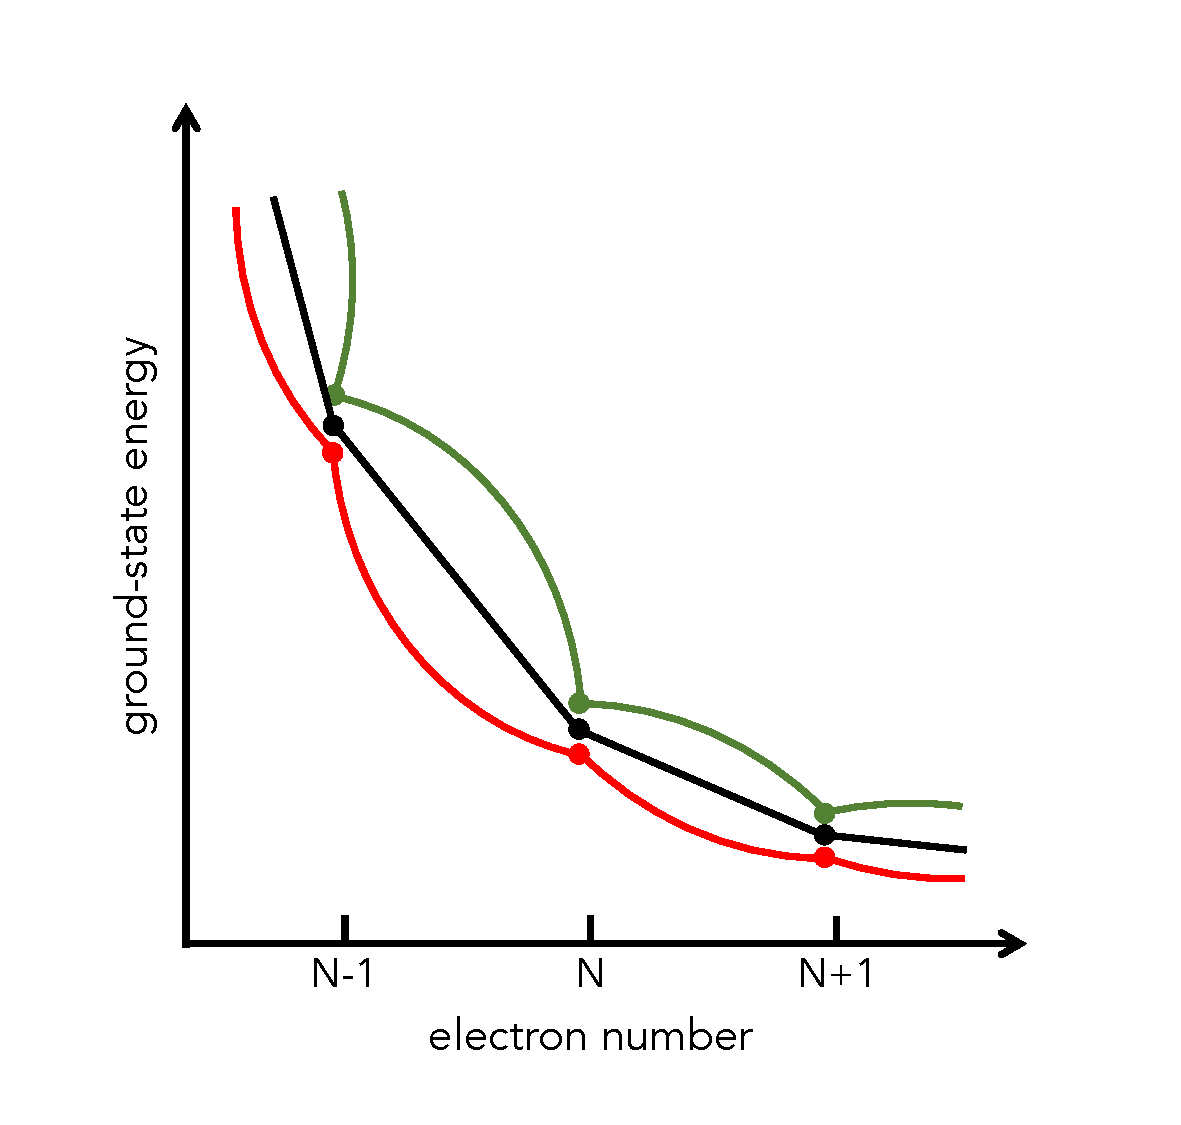
\includegraphics[width=0.5\textwidth]{pwl-exact-approx.pdf}
    \caption[Ground-state energy as a function of the number of electrons: comparison between the exact, the PBE, and the HF curves.]{Ground-state energy at the different levels of approximation. The black line represents the exact piecewise-linear trend, the red line shows the convex behavior of a local (or semi-local) functional such as PBE, and the green curve shows the concave behavior (on each segment connecting consecutive integer points) of the HF energy. The PBE (HF) energy at integer numbers of electrons is placed below (above) the correspondent exact energy, not because of a general underestimation (overestimation), but rather to highlight the fact that they never overlap perfectly with the exact ground-state energy. The PZ energy also is above the exact energy and normally has a concave behavior similar to HF, though often it shows an S-like trend with a slightly convex part followed by a change of curvature at fractional number of electrons \cite{vydrov_tests_2007}.}
    \label{fig:deviation-pwl}
\end{figure}

The failure in the description of the dissociation of the $H_2^+$ molecule, as well as that of other molecules, can be understood also in terms of another error affecting DFAs. In Sec.~\ref{sec:pwl-energy}, we saw that the ground-state energy is a PWL function of the number of electrons; local and semi-local functionals instead display a non-linear convex behavior at fractional occupations, as shown in Fig.~\ref{fig:deviation-pwl}. As a consequence of the convexity, the approximated ground-state energy fulfills the property
%
\begin{equation}
    E \left[ \delta(N-1) + (1-\delta)N \right] < \delta E(N-1) + (1-\delta) E(N) \qquad \qquad
    \text{for} \quad 0 \leq \delta \leq 1 ,
    \label{eq:convexity}
\end{equation}
%
which shows that -- for a (semi-)local functional -- splitting an electron is always energetically convenient. This explains why, in the $H_2^+$ molecule, local functionals gain energy from placing half electron on each hydrogen atom in the limit of large interatomic distances and, in general, fail to describe the dissociation of molecules \cite{vydrov_tests_2007}. The exact correction of the SIE in the one-electron limit, restores the PWL of the energy for $0 \leq N \leq 1$, and allows to describe correctly systems with a fraction of an electron; however, it does not equally implicate a better description at fractional particle numbers also in many-electron systems. On the other hand, those methods in closer agreement with the PWL behavior provide a better description of the dissociation of molecules and, in general, of systems with fractional number of electrons. This observation has encouraged Ruzsinszky and collaborators, to define as \emph{nearly} many-electron SIE-free, functionals that are piecewise linear at \emph{any} particle numbers \cite{ruzsinszky_spurious_2006}.

The deviation from the PWL gives rise also to other errors, one of which is related to static correlations. In systems presenting spin-degenerate ground states, densities with integer and fractional number of electrons in each spin channel can be energetically equivalent, and this can be directly linked to the piecewise-linear character of the energy. In local and semi-local functionals -- but also in non-local methods like Hartree-Fock and hybrid functionals (see Sec.~\ref{sec:non-local}) -- the non-linear behavior of the energy brings to a systematic overestimation of the energy for spin-densities with fractional number of electrons \cite{cohen_fractional-spins_2008, cohen_insights_2008}. The \emph{static correlation error} explains the overestimation of dissociation energies of molecules like $H_2$, and normally its magnitude increases with the number of bonds in the system.

With respect to charged excitations, the PWL plays a key role for the correct prediction of the ionization energies. From Janak's theorem (Eq.~\eqref{eq:janak-th}), and by means of the Aufbau principle, one can easily show that the left derivative of the energy with respect to the number of particles is $\varepsilon_{\rm HO}$. The convex non-linear behavior of local functionals, creates a discrepancy between total and differential energy differences -- with the latter matching $\varepsilon_{\rm HO}$ -- which explains the systematic underestimation of IPs from local and semi-local functionals.

\section{Non-local potentials\label{sec:non-local}}
The KS potential represents the variationally best local and static approximation to the electronic self-energy \cite{casida_generalization_1995}, and allows to determine some of the collective properties of the system (ground-state density, total energy, etc.). With a few exceptions, the single-particle properties of the KS system do not have any physical meaning and, in particular, the KS eigenvalues do not seem to have any link with the ionization energies of the real system. This lack of connection between the KS system and the quasiparticle properties can be traced back to the local nature of the KS effective potential, which cannot mimic the whole complexity of the interaction -- known to be non-local and frequency-dependent -- between a (quasi-)electron and the rest of the system. In this section, we analyze the consequences of replacing the local KS potential (or at least a part of it) with some non-local operator, which normally increases the complexity of the calculations, but also improves the accuracy of the predictions.

Starting with the prototypical non-local approach, the Hartree-Fock system, discussed in Sec.~\ref{sec:hartree-fock}, which represents one of the first effective methods to solve the Schr\"{o}dinger equation of a many-electron system, we will move on to more complex approaches that involve appropriate mixing of the non-local Fock exchange with some local exchange and correlation density-functionals. This hybrid functionals are discussed in Sec.~\ref{sec:hybrids}, and represent one of the state-of-the-art methods for electronic structure calculations.

\subsection{Hartree-Fock system and Koopmans' theorem\label{sec:hartree-fock}}
In 1928, D. R. Hartree proposed a method, that he called \emph{self-consistent field}, to solve the Schr\"{o}dinger equation of an atom \cite{hartree_wave_1928}, starting from a wave function given by the simple product of one-electron orbitals. Two years later, J. C. Slater and V. A. Fock pointed out, independently, that the wave function used by Hartree did not satisfy the antisymmetry property of fermions \cite{slater_note_1930, fock_naherungsmethode_1930}. By defining the trial wave function as a Slater determinant, Fock derived the equations that characterize the well-known Hartree-Fock (HF) method. In the following, we show the main steps of the derivation.

Given the set of $N$ single-electron orbitals $\{ \phi_i \}$, we define the many-body wave function as a Slater determinant (once again, for simplicity, we consider a spin unpolarised system and omit the spin indices):
%
\begin{equation}
    \Psi(\br_1, \dots, \br_N) = \frac{1}{\sqrt{N!}}
    \begin{vmatrix}
        \phi_1(\br_1) & \phi_2(\br_1) & \cdots & \phi_N(\br_1) \\
        \phi_1(\br_2) & \phi_2(\br_2) & \cdots & \phi_N(\br_2) \\
        \vdots & & \ddots & \vdots \\
        \phi_1(\br_N) & \phi_2(\br_N) & \cdots & \phi_N(\br_N)
    \end{vmatrix} ,
    \label{eq:slater-determinant}
\end{equation}
%
while the expectation value of the electronic Hamiltonian over $\Psi$ defines the HF energy functional $E^{\rm HF}[\Psi]$. Thanks to the Rayleigh-Ritz variational principle, the energy minimum can be found by deriving the HF functional with respect to the one-electron wave functions. When the orthonormality constraint on the $\{ \phi_i \}$ is imposed, the minimization problem reduces to the set of well-known \emph{Hartree-Fock equations}:
%
\begin{equation}
    \left[ -\frac{\nabla^2}{2} + v_{\rm H}([\rho],\br) - v_{\rm x}([\gamma],\br) + v(\br) \right] \phi_i(\br) = \varepsilon_i \phi_i ,
    \label{eq:hf-equations}
\end{equation}
%
where $v_{\rm H}$ is the Hartree potential defined in Eq.~\eqref{eq:hartree-potential}, $v$ is the external potential, and $v_{\rm x}$ is the (Fock) exchange potential defined as the gradient of the exchange energy:
%
\begin{equation}
    E_{\rm x} = \frac{1}{2} \sum_{i,j} \int d\br d\br' \frac{\phi_i^*(\br)\phi_j^*(\br)\phi_j(\br')\phi_i(\br')}{|\br-\br'|}
    \label{eq:fock-exchange-energy}
\end{equation}
%
and
%
\begin{equation}
    \left( \hat{v}_{\rm x}[\gamma] \phi_i \right)(\br) = \frac{\delta E_{\rm x}}{\delta \phi_i^*(\br)} = \int d\br' \frac{\gamma(\br,\br') \phi_i(\br')}{|\br-\br'|} ,
    \label{eq:fock-exchange-potential}
\end{equation}
%
with $\gamma(\br,\br')$ being the density matrix, $\gamma(\br,\br') = \sum_j \phi_j^*(\br) \phi_j(\br')$. The presence of the density matrix makes the Fock potential a non-local\footnote{In the sense that the action of the exchange potential on the wave function $\phi(\br)$ at the point $\br=\br'$, depends on the values of $\phi(\br)$ at all the points $\br$; this is not the case of, e.g., the Hartree potential (Eq.~\eqref{eq:hartree-potential}), whose action on $\phi(\br)$ at $\br=\br'$ depends only on the value of $\phi(\br)$ at $\br=\br'$.} -- thus, non-multiplicative -- operator, therefore its explicit expression can be given only when considering the action on some wave function. In this sense, the notation $v_{\rm x}([\gamma],\br)$ used in Eq.~\eqref{eq:hf-equations}, is not strictly correct, whereas one should refer to Eq.~\eqref{eq:fock-exchange-potential}, for a proper definition of the Fock potential. As for the KS system (see Sec.~\ref{sec:hk-ks-theorems}), the HF equations do not represent an eigenvalue problem, since all the equations are coupled through the density (and in this case also the density matrix). The self-consistent field method devised by Hartree, allows to find a solution to Eq.~\eqref{eq:hf-equations} in an iterative way, where at each step the eigenvectors of the effective Hamiltonian define the density (and thus the Hamiltonian) at the following step; the minimization problem is solved when the self-consistent field method reaches convergence, that is when there are no differences in the eigenvectors (or eigenvalues) between two consecutive steps. The power of this method, is that it is not restricted to the HF theory, but to all those systems that have a similar coupling between the operator and its (quasi-)eigenvectors, the KS system being an example.

As mentioned at the beginning of this section, in its initial formulation, Hartree did not account for the principle indistinguishability of particles, and the wave function was a simple product of the single-electron orbitals. The equations obtained by Hartree differ from those in \eqref{eq:hf-equations} by the Fock term only (from which the name ``Hartree'' for the other Coulomb integral), while the exchange potential appears only when the many-body wave function is turned into an antisymmetric linear combination of all the possible permutations of the $N$ single-electron orbitals. The exchange interaction, then, is a pure result of the quantum nature of particles, and it has a crucial impact on the physical properties of the system, the most important being the self-interaction freedom. In fact, if we look at the explicit expression of the HF energy in terms of the one-electron orbitals,
%
\begin{equation}
    E^{\rm HF}[\{ \phi_i \}] = \sum_i \braket{\phi_i|\hat{h}_0|\phi_i} + \frac{1}{2} \sum_{i,j} \left( \left\langle \phi_i\phi_j \left| \frac{1}{|\hat{\br}_1-\hat{\br}_2|} \right| \phi_i\phi_j \right\rangle
    - \left\langle \phi_i\phi_j \left| \frac{1}{|\hat{\br}_1-\hat{\br}_2|} \right| \phi_j\phi_i \right\rangle
    \right) ,
    \label{eq:hf-energy}
\end{equation}
%
-- where $\hat{h}_0$ embodies the non-interacting part of the Hamiltonian -- the self-Hartree and self-exchange terms of each orbital (corresponding to $i=j$ in the second sum) cancel each other out. This particular feature of the Fock exchange of restoring an exact property of the system inspired the formulation of the so-called \emph{hybrid functionals}, discussed in the next section.

The Hartree-Fock system is endowed with another important property, regarding its eigenvalues. Differently from what happens in the KS system where, generally, eigenvalues and eigenvectors do not have any particular physical meaning, the HF system benefits from a theorem formulated by T. Koopmans in 1934 \cite{koopmans_uber_1934}, that identifies the eigenvalues with the ionization energies of the system. With the assumption that the orbitals do not change when an electron is added to -- or removed from -- the system, Eq.~\eqref{eq:hf-energy} allows to obtain the following expression for the energy difference between the $N$- and $(N-1)$-particle systems
%
\begin{equation}
    E^N - E^{N-1}_i = \braket{\phi_i|\hat{h}_0|\phi_i} + \sum_j^N \left( 
    \left\langle \phi_i\phi_j \left| \frac{1}{|\hat{\br}_1-\hat{\br}_2|} \right| \phi_i\phi_j \right\rangle
    - \left\langle \phi_i\phi_j \left| \frac{1}{|\hat{\br}_1-\hat{\br}_2|} \right| \phi_j\phi_i \right\rangle
    \right) ,
    \label{eq:koopmans-th-intermediate-step}
\end{equation}
%
where the $i$-th orbital has been emptied. Finally, from Eq.~\eqref{eq:hf-equations} we can identify the right-hand side of Eq.~\eqref{eq:koopmans-th-intermediate-step} with the eigenvalue $\varepsilon_i$. In the same way, one can obtain an analogous result for the empty states and complete what is known as \emph{Koopmans' theorem}:
%
\begin{equation}
    \begin{split}
    E^N - E^{N-1}_i &= \varepsilon_i \\
    E^{N+1}_i - E^N &= \varepsilon_i .
    \end{split}
    \label{eq:koopmans-theorem}
\end{equation}
%
We point out that, while in most of the textbooks Koopmans' theorem is proven for the eigenstates of the HF Hamiltonian, the same result applies to any other representation yielding the ground-state density. This can be easily obtained by starting from the HF equations, written for a given set of orbitals differing from the canonical ones and applying the same derivation discussed before. Provided that the energies $E^{N \pm 1}_i$ correspond to the system where the $i$-th orbital of the \emph{new} basis has been emptied/filled, Koopmans' theorem for a non-diagonal representation reads as
%
\begin{equation}
    \begin{split}
    E^N - E^{N-1}_i &= \Lambda_{ii} \\
    E^{N+1}_i - E^N &= \Lambda_{ii} ,
    \end{split}
    \label{eq:koopmans-theorem-noncanonical}
\end{equation}
%
where $\Lambda_{ii}$ are the diagonal elements of the matrix of Lagrange multipliers.

The biggest drawback of HF theory is the total neglect of electronic correlations, with the exception of the exchange energy. Although resorting to the exact Hamiltonian, the wave function used is a single Slater determinant, which is far from being a complete set of wave functions and loses track of most of the interactions between electrons. Thanks to its freedom from the SIE, HF theory provides a better qualitative description of processes involving fractional number of electrons, such as the dissociation of molecules \cite{ruzsinszky_spurious_2006}; on the other hand, the lack of correlation brings to a much larger static correlation error with respect to local density-functionals \cite{cohen_fractional-spins_2008}, and to a concave deviation from the piecewise-linearity (see Fig.~\ref{fig:deviation-pwl}) when the orbitals are allowed to relax \cite{li_piecewise_2017}. This latter behavior, in particular, is associated with a \emph{localization error}, that is the tendency to overlocalize the orbitals (especially in extended systems) \cite{mori-sanchez_localization_2008}, and it is responsible for the systematic overestimation of ionization potentials (with a mean absolute error above 0.6 eV \cite{colonna_koopmans-compliant_2019}) and underestimation of electron affinities, with a consequent strong overestimation of band gaps.

The accuracy of HF is drastically improved by quantum chemistry multireference methods, that recover part of the electronic correlation by realizing wave functions that combine several Slater determinants. The most well-known are the \emph{configuration interaction} (CI) and \emph{coupled cluster} (CC) methods, that augment -- linearly and exponentially, respectively -- the HF wave function with Slater determinants containing single and double (CISD, CCSD), or triple (CCSD(T)) excitations. CI and CC are among the most accurate methods for electronic-structure calculations, and are often taken as a reference for other approaches; however, their poor scaling properties -- CCSD scales like $\mathcal{O}(N^6)$ and CCSD(T) like $\mathcal{O}(N^7)$ -- limit the applications to relatively small molecular systems. For this reason, less complex methods that rather go towards the computational simplicity of DFT are often preferred: hybrid functionals take advantage of some of the features of HF, by mixing the Fock exchange with contributions from local or semi-local functionals, and proved to be one of the best compromises between computational complexity and accuracy for the calculation of excited-state properties.

\subsection{Hybrid functionals\label{sec:hybrids}}
The Hartree-Fock exchange is exact in single-reference methods: for many-body wave functions that can be represented via a Slater determinant, Eq.~\eqref{eq:fock-exchange-potential} represents the exact exchange energy. Inevitably, this stimulated the idea of using the HF exchange to model the exchange part of the xc energy in DFT. Its non-local nature pushes the exact exchange out of the boundaries of Kohn-Sham density-functional theory, which requires potentials that are local in space, and therefore demands for alternative approaches, such as the optimized effective potential method or the generalized Kohn-Sham scheme (discussed later in this section). Because of some cancellation of (self-interaction) errors that normally occurs when using consistent exchange and correlation functionals \cite{vydrov_effect_2004}, the straight replacement of the local approximate exchange energy with the exact exchange, usually worsens the quality of the results. However, an appropriate mixing of the HF and local, or semi-local, exchange energies can dramatically improve the performance of standard density-functional approximations.

By means of the adiabatic connection formula, A. D. Becke introduced a rigorous way to include the exact exchange in the definition of the xc energy \cite{becke_new_1993}. Following his reasoning, let us consider the collection of many-body wave functions $\{ \Psi_{\lambda} \}$, all yielding the ground-state density $\rho$ of the real system, with $\lambda$ representing the coupling parameter that gauges the strength of electronic interaction ($\lambda=0$ corresponds to the non-interacting system, $\lambda=1$ to the fully interacting one); then, the exact xc energy can be defined as (see also Appendix~\ref{app:xc-hole})
%
\begin{equation}
    E_{\rm xc} = \int_0^1 d\lambda E_{{\rm xc},\lambda} = \int_0^1 d\lambda \braket{\Psi_{\lambda}|\hat{V}_{\rm ee}|\Psi_{\lambda}} - E_{\rm H}[\rho] .
    \label{eq:adiabatic-connection}
\end{equation}
%
Becke noticed that, in the non-interacting limit, the wave function reduces to the Kohn-Sham Slater determinant -- like HF, KS theory is, indeed, a single-reference method -- and $E_{{\rm xc},0}$ becomes the exact exchange energy of the KS system. On the other hand, when $\lambda$ approaches 1, we find that $E_{{\rm xc},\lambda}$ is the xc energy of the fully interacting system, that can be approximated with, e.g., local or semi-local functionals. The complete $\lambda$ dependence of $E_{{\rm xc},\lambda}$ is, of course, unknown and approximations are normally needed: Becke's ``half-and-half'' hybrid resulted from the linear interpolation of the $E_{{\rm xc},0}$ and $E_{{\rm xc},1}$ points, where the upper bound was approximated by the LSDA xc energy, and showed a significant improvement with respect to HF and LSDA \cite{becke_new_1993}.

Thereafter, Perdew, Ernzerhof and Burke considered a more general polynomial interpolation and, by comparison with M\o{}llet-Plesset perturbation expansion, they estimated the general optimal power expansion at the fourth order \cite{perdew_rationale_1996}. This gave birth to the mixing of PBE and exact exchange defining the well-known PBE0 hybrid functional
%
\begin{equation}
    E_{\rm xc}^{\rm PBE0} = \frac{3}{4} E_{\rm x}^{\rm PBE} + \frac{1}{4} E_{\rm x}^{\rm HF} + E_{\rm c}^{\rm PBE} .
    \label{eq:pbe0-hybrid}
\end{equation}
%
Among the several recipes available in the literature, here we mention another commonly used hybrid, namely the Becke, 3-parameter, Lee-Yang-Parr (B3LYP) xc functional \cite{becke_densityfunctional_1993,stephens_ab_1994}, that reads as
%
\begin{equation}
    E_{\rm xc}^{\rm B3LYP} = (1-a_0) E_{\rm x}^{\rm LSDA} + a_0 E_{\rm x}^{\rm HF} + a_{\rm x} \Delta E_{\rm x}^{B88} + (1-a_{\rm x}) E_{\rm x}^{\rm LSDA} + a_{\rm c} E_{\rm c}^{\rm LYP} ,
    \label{eq:b3lyp-hybrid}
\end{equation}
%
where $\Delta E_{\rm x}^{B88}$ is Becke's gradient correction and $E_{\rm c}^{\rm LYP}$ is the Lee-Yang-Parr correlation functional \cite{lee_development_1988}. The optimal values for the three semi-empirical parameters are $a_0 = 0.20$, $a_{\rm x} = 0.72$, $a_{\rm c} = 0.81$, and were obtained by fitting several thermodynamic quantities on a set of atoms and molecules.

As mentioned earlier in this section, the inclusion of the HF exchange energy within the expression for the xc functional does not go along with the KS formulation. The exact exchange is orbital-dependent -- in the sense that it depends explicitly on the orbitals, rather than the total density -- and its gradient provides an operator that violates the condition of locality of the KS mapping. Nevertheless, since any set of KS orbitals is uniquely defined by some ground-state density, HK theorem implies that the HF exchange energy calculated on those orbitals is a functional -- although implicit -- of the total density. The \emph{optimized effective potential} (OEP) method \cite{sharp_variational_1953,talman_optimized_1976} defines a set of integral equations -- which is nothing more than a linearized Sham-Schl\"{u}ter equation \cite{sham_density-functional_1983} -- that allow to calculate the functional derivative of the exchange energy (with respect to the total density), and finds the best variational local potential corresponding to some non-local scheme. The effective Hamiltonian is then KS-like with the potential determined by the equation of the OEP method. Thanks to their local nature, OEPs are much simpler both conceptually and computationally, and they normally predict properties in close agreement with their orbital-dependent analogous \cite{kummel_orbital-dependent_2008}. Yet, solving the integral equations to determine the optimal local potential, is a rather complicate task and sometimes it can be more convenient to address the problem by considering the explicit orbital dependence.

A different approach that instead retains the non-locality of the exact exchange potential and actually benefits from it, is the \emph{generalized Kohn-Sham} (GKS) scheme \cite{seidl_generalized_1996}. Differently from KS theory, which treats exactly only the non-interacting part of the system -- namely, $T_0$, $E_{\rm H}$ and $V_{\rm ext}$ -- and piles up all the rest in the exchange-correlation energy, in the GKS scheme part of the electronic correlation (usually the exchange) is included in the functional $S[\{ \phi_i \}]$, whose explicit dependence on the one-electron orbitals allows to incorporate quantities such as the Fock exchange (as well as other expressions including a fraction of it, such as the aforementioned PBE0 and B3LYP functionals). The total energy reads as
%
\begin{equation}
    E[\rho] = F^{S}[\rho] + \int d\br \rho(\br) v(\br) + R^{S}[\rho] ,
    \label{eq:gks-energy}
\end{equation}
%
where $F^{S}[\rho]$ is the functional minimizing $S[\{ \phi_i \}]$, provided that the orbitals $\{ \phi_i \}$ yield the density $\rho$, while the remainder functional $R^{S}[\rho]$ embodies the rest of the correlation. Upon application of the variational principle, with the usual Lagrange multipliers ensuring the orthogonality of the orbitals, we obtain the following set of GKS equations:
%
\begin{equation}
    \left( \hat{O}^S[\{ \phi_i \}] + v(\br) + v^R(\br) \right) \phi_i(\br) = \varepsilon_i \phi_i(\br) ,
    \label{eq:gks-equations}
\end{equation}
%
where $(\hat{O}^S \phi_i)(\br) = \delta S[\{ \phi_i \}] / \delta \phi_i(\br)$, and $v^R(\br) = \delta R^S[\rho] / \delta \rho(\br)$. Depending on the choice of the functional $S[\{ \phi_i \}]$, different schemes can be obtained: for instance, when $S[\{ \phi_i \}]$ is simply given by the (non-interacting) kinetic energy $T_0$ the standard KS equations are obtained, while the inclusion of the Hartree and Fock energies provides the so-called Hartree-Fock Kohn-Sham scheme \cite{seidl_generalized_1996}.

In Sec.~\ref{sec:deriv-dis} we saw that in KS-DFT, even for the exact functional, the KS band gap does not capture all the contributions to the real band gap, whereas one needs to calculate explicitly also the discontinuity of the xc potential. Actually, this issue affects any scheme characterized by a local effective potential, therefore, also the eigenvalues resulting from the OEP method -- which is, in effect, a KS scheme resulting from an orbital-dependent functional -- do not embody any part of $\Delta_{\rm xc}$. However, differently from local functionals for which $\Delta_{\rm xc}$ is identically zero, orbital-dependent functionals generally have a derivative discontinuity that can be, in principle, summed up to the KS-OEP band gap. One of the advantages of generalized Kohn-Sham schemes is that part of the derivative discontinuity is embodied in the eigenvalues. As shown by Seidl \emph{et al.}, thanks to the explicit orbital-dependence of the exact exchange, the derivative discontinuity of the exchange energy enters in the difference between the HO-LU GKS eigenvalues \cite{seidl_generalized_1996}. Since the exchange part of the derivative discontinuity is often dominant, the GKS band gap normally matches quite well with the differential band gap. This has been showed, e.g., in Ref.~\cite{cohen_fractional-charge_2008}, where the comparison between the GKS eigenvalues and OEP derivatives -- i.e., the sum of OEP-KS eigenvalues and the xc energy derivatives -- showed a good agreement for IP, EA and band gap for both Hartree-Fock and the MCY3 hybrid functional, with the latter reproducing accurately also the experimental values thanks to its almost exact piecewise-linear nature. The good agreement with the experiment, not only for the calculated band gaps, but also for IPs and EAs, is an indicator of the physical connection between GKS eigenvalues corresponding to frontier orbitals and first ionization energies \cite{perdew_understanding_2017}. Besides, the relative position of other quasiparticle energies with respect to the HO and LU levels -- i.e., the bandwidth in crystalline materials -- generally, is qualitatively the same between local, semi-local, and hybrid functionals, other more advanced approaches such as the GW method discussed in Sec.~\ref{sec:gw} and, ultimately, the experiment. This means that a method that opens the band gap, by shifting correctly the absolute position of both the HO and LU levels, often predicts also the rest of the spectrum with good accuracy.

In the last decade a class of hybrid functionals involving a screened version of the exact exchange via a spatial separation of active and inactive regions, has achieved resounding success, especially when dealing with extended periodic systems. The idea behind these so-called \emph{range-separated hybrids} (RSH), is based on the fact that local and semi-local functionals model quite well the short-range part of the Coulomb interaction, whereas they miss the long-range contribution to the xc energy. On the other hand, the non-local character of orbital-dependent functionals allows to capture more effectively the long-range interactions. Therefore, it was suggested to separate the Coulomb interaction in a short- and a long-range contributions as
%
\begin{equation}
    \frac{1}{|\br-\br'|} = \frac{\erf(\gamma |\br-\br'|)}{|\br-\br'|} + \frac{\erfc(\gamma |\br-\br'|)}{|\br-\br'|} ,
    \label{eq:range-separation-coulomb}
\end{equation}
%
with $\erf(x)$ being the error function and embodying the long-range (LR) component, and $\erfc(x) = 1 - \erf(x)$ the complementary error function for the short-range (SR) part; the parameter $\gamma$ determines the spatial extension of the two regions. A well-known RSH, is the Heyd-Scuseria-Ernzerhov (HSE) functional \cite{heyd_hybrid_2003}, which generalizes the PBE0 functional in the following way:
%
\begin{equation}
    E_{\rm xc}^{\rm HSE} = a E_{\rm x}^{\rm HF,SR}(\gamma) + (1-a) E_{\rm x}^{\rm PBE,SR}(\gamma) + E_{\rm x}^{\rm PBE,LR}(\gamma) + E_{\rm c}^{\rm PBE} ,
    \label{eq:hse-hybrid}
\end{equation}
%
where $E_{\rm x}^{\rm HF,SR}(\gamma)$, $E_{\rm x}^{\rm PBE,SR}(\gamma)$ and $E_{\rm x}^{\rm PBE,LR}(\gamma)$, represent the short-range HF exchange and the short- and long-range components of the PBE exchange energy, respectively. The functional HSE06 is characterized by the same choice of PBE0 for the mixing parameter, $a=1/4$, and the value of 0.2 for the range-separation parameter $\gamma$, while for $\gamma=0$ HSE retrieves the PBE0 functional.

One of the issues with hybrid functionals is the fact that results can be strongly affected by the values of the mixing parameters. Just like the energy, the mixing parameters are functionals of the density rather than simple numbers, and the choice of a global value cannot be effective for all the systems. Hybrid functionals, whose parameters are determined semi-empirically via fitting of experimental results, can be rather accurate for specific properties in a range of materials, but the failure to describe other physical features is inevitable. For this reason, recent works analyzed the possibility of having system-dependent parameters that are determined from first-principles, either via the imposition of exact constraints, or by analogy with higher-level theories. The compliance with the DFT version of Koopmans' theorem, introduced in Sec.~\ref{sec:hk-ks-theorems}, is one of the exact constraints that helped to develop accurate RSHs for the prediction of band gaps both in molecules and solids. In this case the range-separation parameter $\gamma$ is determined via the minimization of the deviation of the GKS frontier eigenvalues from the corresponding ground-state energy differences \cite{stein_fundamental_2010,refaely-abramson_quasiparticle_2012}:
%
\begin{equation}
    J(\gamma) = \left| \varepsilon_N^{\rm GKS}(\gamma) + E(N-1;\gamma) - E(N;\gamma) \right| + \left| \varepsilon_{N+1}^{\rm GKS}(\gamma) + E(N;\gamma) - E(N+1;\gamma) \right| ,
    \label{eq:kc-condition-hybrids}
\end{equation}
%
sometimes replaced by a least squares deviation, rather than a linear one. From a practical point of view, $\varepsilon_{N+1}^{\rm GKS}$ can be taken to be the LU eigenvalue of the $N$-electron system, rather than the -- more correct -- HO eigenvalue of the $(N+1)$-electron system: as long as the missing derivative discontinuity in the GKS eigenvalues is small, such approximation is reliable. Besides, the balance of local and non-local components resulting from this Koopmans' condition, yielded functionals with an improved PWL character. Moreover, such condition has been successfully employed also in global hybrids (lacking of range-separation), to determine the intra-gap levels of point defects -- including interstitial and substitutional defects, and polaronic distortions -- in extended systems \cite{miceli_nonempirical_2018,bischoff_adjustable_2019}.

Another aspect, especially important for band gap calculations, is the asymptotic behavior of the Coulomb potential. As mentioned in Sec.~\ref{sec:errors-dft}, due to the cancellation, at large distances, of the Hartree and external potentials, the xc potential should decay as $-1/r$ (in the gas phase), whereas local potentials display an exponential decay. The full HF exchange potential has precisely this asymptotic behavior, therefore, the mixing parameters are often chosen in a way that makes the prefactor of the HF term equal to one in the long-range limit. In extended systems, screening effects become significant, and the mixing parameters of the hybrid functional are chosen to satisfy the renormalized asymptotic behavior $-1/(\varepsilon r)$ \cite{refaely-abramson_gap_2013}, with $\varepsilon$ representing the scalar dielectric constant of the material. A further step in this direction was made by Skone and collaborators, who pointed the similarities between the expression of the exchange-correlation potential coming from a generic hybrid functional, and the electron self-energy in the static \gw approximation \cite{skone_self-consistent_2014}.
The identification of the mixing parameters with the dielectric constant has been applied to both global \cite{miceli_nonempirical_2018,skone_self-consistent_2014} and range-separated \cite{skone_nonempirical_2016,chen_nonempirical_2018} hybrids giving rise to the so-called \emph{dielectric-dependent hybrid} (DDH) functionals. Sometimes this has been also combined with the Koopmans' condition to determine the other parameters tuning the long- and short-range mixing of local and exact exchange \cite{refaely-abramson_gap_2013}, showing an accuracy comparable to state-of-the-art many-body perturbation theory methods.

Finally, we mention that in extended periodic systems, in order to have meaningful mixing parameters, it is of pivotal importance to overcome (or avoid) the delocalization error mentioned in Sec.~\ref{sec:deriv-dis}. Due to the delocalized nature of the electronic states, the energy displays a wrong piecewise-linear behavior where each linear segment has a slope that strongly overestimates the exact one. Eq.~\eqref{eq:kc-condition-hybrids} is then trivially solved for any value of $\gamma$. GKS electrons must then ``sit'' on localized orbitals, and this has been realized by employing potential probes that force the localization of the highest-occupied state \cite{bischoff_adjustable_2019,yang_one-shot_2022}, or by replacing the natural (delocalized) Bloch-like representation of the electronic states with a localized set of orbitals, namely the Wannier functions \cite{wing_band_2021}. The latter approach has been adopted also within the framework of Koopmans spectral functionals and, as discussed in detail in the following chapters, it is fundamental to have meaningful corrections of local and semi-local functionals.

\section{Green's function methods\label{sec:green-function-methods}}
In the last part of this chapter, we take a further step forward in the description of the effective interactions experienced by the (quasi-)electrons, and consider approaches that account not only for the static -- although non-local -- components of the electronic correlation, but also for its dynamical part. The prototypical tool for treating the interaction of a many-electron system via the quasiparticle picture is the Green's function, which takes the place of the many-body wave function and the total electronic density as the system's descriptor. The problem of solving the electronic Hamiltonian of Eq.~\eqref{eq:many-electron-problem}, is mapped into the determination of the Green's function of the system, whose solution can be found perturbatively by means of \emph{many-body perturbation theory} (MBPT). In the following we will give a brief overview of MBPT and of one of its infamous applications, the GW approximation, to highlight the key features that are relevant within this dissertation, while for a more detailed description we refer to the huge variety of textbooks and reviews available in the literature. In particular, the concepts discussed in this section are mainly taken from Refs.~\cite{martin_interacting_2016,fetter_quantum_1971,reining_gw_2018,onida_electronic_2002}

Before introducing the Green's function, we want to point out the origin of the presence of a dynamical component -- totally absent in the time-independent many-body Schr\"{o}dinger equation \eqref{eq:many-electron-problem} -- in the description of the effective electronic interaction. Following Ref.~\cite{martin_interacting_2016}, let us imagine to split the problem into two sub-systems: a small part, representing the system that we want to solve -- e.g. an electron\footnote{Here, as well as in other parts of this thesis, we often speak about electrons rather than quasi-electrons. Of course, the concept of electron within an interacting system loses importance, and we may alternatively refer to it when dealing with non-interacting systems, or when implicitly considering its quasiparticle version. We leave to the reader the correct interpretation.} -- and a remainder part, i.e. the bath, whose interaction with the small part needs to be accounted for. The eigenvalue problem reads as
%
\begin{equation}
    \begin{pmatrix}
        H_S & H_{S-b} \\
        H_{b-S} & H_b
    \end{pmatrix}
    \begin{pmatrix}
        \psi_S \\
        \psi_b
    \end{pmatrix} =
    \omega
    \begin{pmatrix}
        \psi_S \\
        \psi_b
    \end{pmatrix}
    \label{eq:frequency-dependence}
\end{equation}
%
where $H_S$ and $H_b$, represent the bare Hamiltonians of the (small) system and the bath, respectively, while $H_{S-b}$ and $H_{b-S}$ model the coupling between the two. It is straightforward to recast Eq.~\eqref{eq:frequency-dependence} into the following non-linear problem for $\psi_S$:
%
\begin{equation}
    \left( H_S + H_{S-b}(\omega - H_b)^{-1}H_{b-S} \right) \psi_S = \omega \psi_S ,
    \label{eq:quasiparticle-equation}
\end{equation}
%
which is called \emph{quasiparticle equation}. The second term between the brackets on the left-hand side, represents the self-energy, $\Sigma(\omega)$, of the system, which is a frequency-dependent operator that embodies the effective interaction between the system and the bath, i.e. between the quasi-electron and the rest of the system. We observe that, when there is no interaction between the bath and the system ($H_{S-b} = H_{b-S} = 0$), the self-energy is zero, the frequency-dependence disappears, and Eq.~\eqref{eq:quasiparticle-equation} turns into a standard eigenvalue problem. It becomes clear then, that the frequency-dependence is a direct consequence of the coupling of the system with the bath; despite the static character of Eq.\eqref{eq:many-electron-problem}, the price to pay in order to describe the interacting many-electron system from a single-particle point of view, is to introduce an effective field, the self-energy, that accounts for the whole interaction via an additional parameter, the frequency.

Although the expectation value of any observable is a functional of the density (thanks to HK theorem), explicit expressions are often difficult (if not impossible) to find. Many of these observables -- and, particularly, spectral properties -- have a more accessible form, at least in principle, in terms of the Green's function. The latter is an object which is non-local both in space and time and is designed to capture more effectively the screening effects (i.e. the response of the system) due to the presence of a perturbation, i.e. the potential generated by an electron. Formally, a Green's function is defined as
%
\begin{equation}
    G(x,t;x',t') = -i \braket{\Psi|T[\hat{\psi}(x,t) \hat{\psi}^{\dagger}(x',t')]|\Psi} ,
    \label{eq:green-function}
\end{equation}
%
where $\Psi$ represents the ground state of the $N$-electron system, $T$ is the time-ordering operator, and $\hat{\psi}(x,t)$ and $\hat{\psi}^{\dagger}(x',t')$ are the field operators that, respectively, annihilate a particle at the point $(x,t)$ and create an identical one at the point $(x',t')$. In this notation, $x$ generally embodies spatial and spin coordinates, $x=(\br,\sigma)$. Eq.~\eqref{eq:green-function} emphasizes the physical meaning of the Green's function: a correlation function (similar to Eq.~\eqref{eq:pair-corr-function}), that provides the probability amplitude of finding a particle at $(x,t)$ upon addition of a particle at $(x',t')$. Besides, this is done in the two temporal directions (thanks to the presence of the time-ordering operator), which is totally equivalent to consider the propagation of both electrons and holes. The Green's function, then, traces the evolution of a particle accounting for the (temporal) response of the system and how this affects the particle itself; dynamical correlation is directly encoded in the Green's function, which makes it an ideal descriptor of the dynamics of a particle within an interacting system.

At equilibrium, the time dependence reduces to $t-t'$ and, by Fourier transforming Eq.~\eqref{eq:green-function}, we obtain the Lehmann representation of the Green's function
%
\begin{equation}
    G(x,x',\omega) = \sum_k \frac{f_k^*(x') f_k(x)}{\omega - \varepsilon_k - i\eta \sign(\mu - \varepsilon_k)} ,
    \label{eq:lehmann-representation}
\end{equation}
%
where the set of $\varepsilon_k$ represents the energy differences $E(N)-E_k(N-1)$ and $E_k(N+1)-E(N)$ between the $N$-particle ground state and the $(N\pm 1)$-particle excited states, $\mu$ is the chemical potential, $\eta$ is a small real that ensures the convergence of the Fourier transform, and the quantities at the numerator are the so-called Lehmann amplitudes:
%
\begin{equation}
    f_k(x) = \begin{cases}
        \braket{\Psi^{N-1}_k|\hat{\psi}(x)|\Psi^N_0} , \quad \varepsilon_k < \mu \\
        \braket{\Psi^{N}_0|\hat{\psi}(x)|\Psi^{N+1}_k} , \quad \varepsilon_k > \mu
    \end{cases} .
    \label{eq:lehmann-amplitudes}
\end{equation}
%
Eq.~\eqref{eq:lehmann-representation} is extremely relevant as it highlights immediately an important property of Green's functions, namely its poles correspond to the ionization energies of the system. Actually, much more information about the spectral properties can be directly extracted from the Green's function: its imaginary part provides the \emph{spectral function}
%
\begin{equation}
    A(x,x',\omega) = \frac{1}{\pi} \left| {\rm Im}[G(\omega)] \right| = \sum_k f_k^*(x') f_k(x) \delta(\omega-\varepsilon_k) ,
    \label{eq:spectral-function}
\end{equation}
%
a quantity that is strictly connected to the photoelectron current -- the current of electrons (holes) leaving the system with a certain kinetic energy, upon absorption (emission) of photons of frequency $\omega$ -- and contains, alone, all the information about the (direct and inverse) photoemission spectrum. In the non-interacting limit, many-body wave functions can be represented via single Slater determinants: the Lehmann amplitudes turn into one-electron spin-orbitals and the spectral function, represented onto the basis of eigenvectors, is a diagonal matrix whose elements are delta functions centered on the energies $\varepsilon_k$. The trace of the spectral function corresponds to a series of peaks with no width (infinite quasiparticle lifetime), which portrays exactly the spectrum of a system of non-interacting electrons. As soon as the interaction is switched on, the many-body wave functions cannot be represented anymore by single Slater determinants, but rather by linear combinations of those; the number of non-zero Lehmann amplitudes increases, with the latter losing their mutual orthogonality in order to conserve the number of particles. The $\delta$-like peaks appearing in the spectral function group together and form structures of finite width and height\footnote{In a finite system, in principle, one can always distinguish the individual $\delta$-like spikes forming a broadened peak; in the thermodynamic limit, the distance (which is proportional to the system size) between the individual $\delta$-peaks becomes infinitesimal, and the whole structure takes an actual continuous shape.} that, normally, connect continuously to the isolated (non-interacting) $\delta$-peaks, as long as the switching-on of the interaction is performed adiabatically. These structures represent the quasiparticles peaks, and are centered around the poles of the Green's function. The broadening is an effect that purely stems from the electronic interaction and is directly connected to the finite quasiparticle lifetime. Additionally, the spectral function can display other features resulting from the scattering of the excited electron from the rest of the system, which redistributes the spectral weight of the quasiparticle in smaller and more spread structures called satellites. This was to show that the knowledge of the spectral function is sufficient to have a full description of photoemission spectra, an important ingredient in the discussion that sees orbital-density-dependent potentials as approximations to the spectral potential, and that will be recalled in Sec.~\ref{sec:koopmans-vs-mbpt}.

Besides all its incredible properties, the exact form of the Green's functions is, in general, not known and even computing approximated versions of it can be quite a challenging task. If one starts from the Hartree-Fock approximation, the Lehmann amplitudes are simply the HF eigenvectors and the right-hand side of Eq.~\eqref{eq:lehmann-representation} corresponds to the spectral representation of the operator $(\omega-H^{\rm HF})^{-1}$. The general Green's function has an additional term which accounts for the missing correlation and reads as
%
\begin{equation}
    G(x,x',\omega) = \left[ \delta(x-x') (\omega - H_0(x)) - \Sigma(x,x',\omega) \right]^{-1} ,
    \label{eq:dyson-equation}
\end{equation}
%
which is known as \emph{Dyson equation} for $G$, where $H_0(x)$ in the local Hartree Hamiltonian, and $\Sigma(x,x',\omega)$ is the electronic self-energy which includes also the Fock exchange. The solution of Eq.~\eqref{eq:dyson-equation}, or Eq.~\eqref{eq:lehmann-representation}, can be mapped into the following non-linear eigenvalue problem
%
\begin{equation}
    \left( H_0 + \Sigma(\omega) \right) f_k(\omega) = \omega f_k(\omega)
    \label{eq:quasiparticle-equation-self-energy}
\end{equation}
%
whose eigenvectors coincide with the Lehmann amplitudes, while the eigenvalues give the ionization energies $\varepsilon_k$. The two provide numerator and denominator of Eq.~\eqref{eq:lehmann-representation} and therefore fully define the Green's function. Eq.~\eqref{eq:quasiparticle-equation-self-energy} is the quasiparticle equation, already introduced at the beginning of this section (see Eq.~\eqref{eq:quasiparticle-equation}) and that we have now derived directly from the Green's function; moreover, this allows to highlight the role of effective dynamical interaction taken over by the self-energy.

\begin{figure}
    \centering
    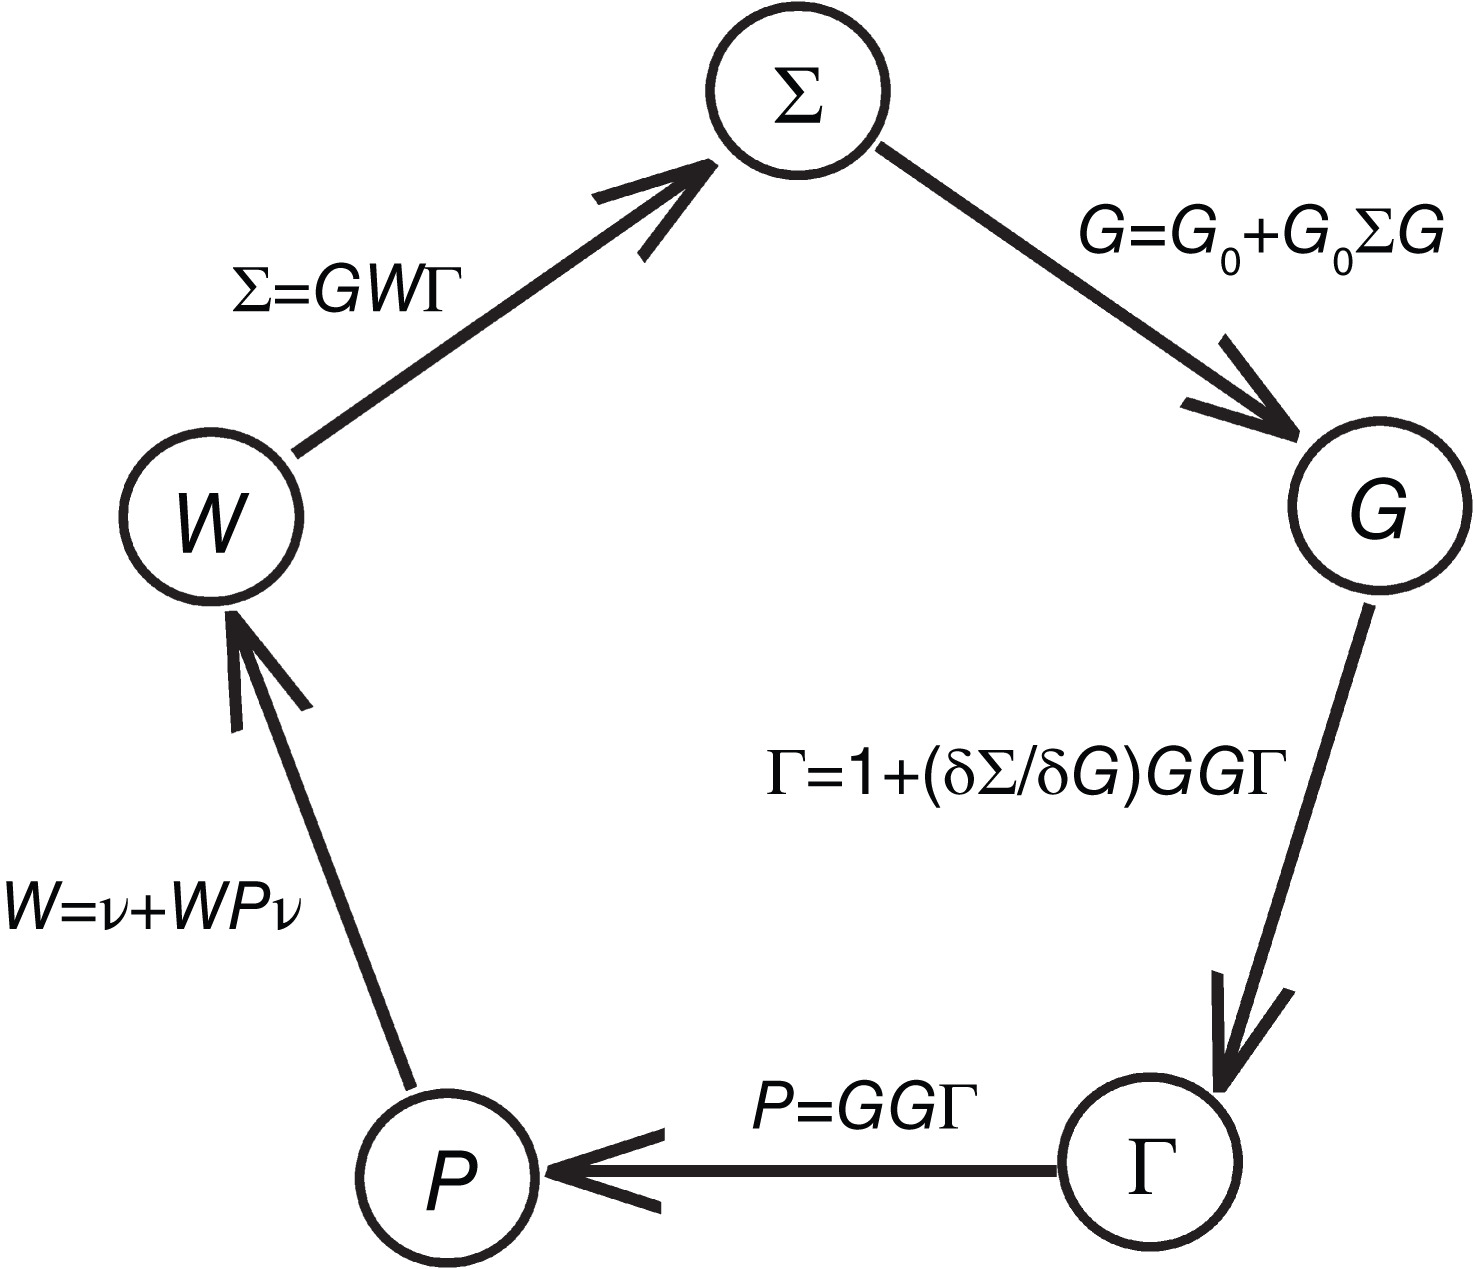
\includegraphics[width=0.5\textwidth]{hedin-equations.jpg}
    \caption[Hedin's set of equations.]{Hedin's loop which includes, in addition to the Dyson equation for $G$, equations for the self-energy ($\Sigma$), the polarizability ($P$), the screened interaction ($W$), and the vertex function ($\Gamma$). Picture taken from Ref.~\cite{leng_gw_2016}.}
    \label{fig:hedin}
\end{figure}

The Dyson equation \eqref{eq:dyson-equation} is a self-consistent equation for the interacting Green's function. The complexity of the problem is transferred to the self-energy: the latter can be expanded in terms of the bare Coulomb interaction and of $G$, and at each perturbation order it gets more ``dressed'' with the response and renormalization of the system. Hedin considered other quantities -- i.e., the polarizability $P$, the screened interaction $W$, and the vertex function $\Gamma$, which contains further information about the electron-hole interaction -- and discovered a closed set of equations (see Fig.~\ref{fig:hedin}) providing a self-consistent scheme that determines the Green's function (as well as the other four quantities involved) of the system. Hedin's equations can be solved iteratively until one reaches, in principle, self-consistency, however such approach is highly non-trivial and computationally expensive. In the following we will see the simplest -- yet very effective -- and most used application of Hedin's equations, yielding the well-known \gw approximation.

\subsection{The \gw approximation\label{sec:gw}}
A possible starting point for the solution of Hedin's equations consists of setting to one the vertex function (actually the vertex is a 3-point function and the approximation is $\Gamma(123)=\delta(12)\delta(13)$). One can use this approximation for $\Gamma$ to obtain an expression for, in order, the polarizability, the screened interaction and, eventually, the self-energy. The latter takes the following form
%
\begin{equation}
    \Sigma^{\gw}(x,x',\omega) = i G(x,x',\omega) W(x',x,\omega)
    \label{eq:gw-approx}
\end{equation}
%
giving the name to the \gw approximation. Such a self-energy can be considered as a dynamically screened generalization of Hartree-Fock theory, whose self-energy is given by the Fock exchange term only and lacks completely of any correlation effects: $\Sigma^{\rm HF} = \Sigma_{\rm x} = i G v$, with $v$ representing the bare Coulomb potential. Once the form of the self-energy is determined, one has still to deal with the non-linear problem of Eq.~\eqref{eq:quasiparticle-equation-self-energy}; often, this is done in a perturbative way, by correcting the eigenvalues of $H_0$ (often taken from some local DFA) with the diagonal elements of the operator $\hat{\Sigma}(\omega) - \hat{v}_{\rm xc}$. The self-energy -- or, more precisely, $G$ and $W$ -- depends on the eigenvalues and different types of approximation can be used depending on how one decides to update the quantities involved. With $G_0 W_0$ one refers to the ``one-shot'' \gw approximation, where the self-energy is not updated and the energies resulting from the first iteration are interpreted as quasiparticles. $G_0 W_0$ is considered a state-of-the-art method for band gap and band structure calculations in solids, as it opens correctly the KS-DFT band gap and delivers accurate predictions, with a general small underestimation of the experimental results. Alternatively, one could update both $G$ and $W$ with the energies obtained at the previous step until reaching self-consistency; this self-consistent \gw method, generally improves total energies and bond lengths but, because of the breaking of some sum rules due to the update of $W^{\rm RPA}$\footnote{The Random Phase Approximation (RPA) is an approximation to the dielectric function -- thus to $W$ -- resulting from the choice $\Gamma(123)=\delta(12)\delta(13)$. Essentially, $W^{\rm RPA}$ is the screened interaction resulting from the \gw approximation.}, it tends to overcorrect the $G_0 W_0$ eigenvalues decreasing the accuracy of photoemission spectra \cite{shishkin_self-consistent_2007}.

Beyond-\gw methods include corrections to the vertex function, which appear already at the second iteration of Hedin's equations. The use of vertex corrections is rather complex, due to wide variety of effects that one can account for, or not, which strongly depend on how they are employed in the Hedin's loop. Self-consistency can also be counter-productive and cancel some of the effects introduced by a non-trivial vertex function. Yet, when used correctly vertex corrections can significantly improve the \gw results and for extended systems, where the system size makes it prohibitive to resort to quantum chemistry multi-reference methods, they provide the most accurate predictions over a large scale of materials \cite{chen_accurate_2015, shishkin_accurate_2007}. In this dissertation, \gw results, with and without vertex corrections, will be often used as a reference to measure the performance of Koopmans functionals.

\clearpage
\section{Summary\label{sec:ch2-summary}}
In this chapter, we discussed two radically different approaches that tackle the many-electron problem: density-functional theory and many-body perturbation theory. In principle, both methods offer an exact way to solve the electronic Hamiltonian \eqref{eq:many-electron-problem}, but, in practice, several approximations are normally required. In DFT, all the observables are depicted via their functional dependence upon the electronic ground-state density, while the whole complexity of the problem is incorporated in the exchange-correlation functional. The KS auxiliary system provides a practical way to obtain collective properties, such as total energies and densities, but its non-interacting particles cannot give a reliable representation of the quasiparticles, whereas the local and static nature of the KS potential makes it impossible to capture all the features of the electronic effective interaction. Generalized KS schemes allow to overcome the constraint of locality on the effective potential, and embrace the possibility of including the Fock non-local exchange within the definition of the potential. The presence of a non-local component brings to a better characterization of the interaction of an electron with the rest of the system, and hybrid functionals considerably improve the prediction of band gaps and higher-order ionization energies. Eventually, the interaction seen from a single-particle point of view brings about dynamical correlation effects, that can be accounted for only by dressing the effective potential with a frequency-dependence. MBPT's self-energy possesses all these features and represents the exact effective interaction that an electron feels inside an interacting many-electron system. Nevertheless, the problem of finding a good self-energy is quite challenging and, ultimately, one would like to reduce the computational complexity of state-of-the-art methods, such as the \gw approximation, while keeping the same level of accuracy (or even improving it).
